\documentclass[12pt,a4paper]{article}
\usepackage[a4paper,margin=25mm]{geometry}
\usepackage[T1]{fontenc}
\usepackage[utf8]{inputenc}
\usepackage{lmodern}
\usepackage{microtype}
\usepackage{amsmath}
\usepackage{amssymb}
\usepackage{graphicx}
\usepackage{booktabs}
\usepackage{hyperref}
\usepackage[backend=biber,style=authoryear,doi=true,url=false,isbn=false,eprint=false]{biblatex}
\addbibresource{references.bib}
\hypersetup{
  colorlinks=true,
  linkcolor=blue,
  citecolor=blue,
  urlcolor=blue
}

\title{The Current Earth Model in \texttt{synthmoon}}
\author{Peter Thejll}
\date{\today}

\begin{document}
\maketitle

\begin{abstract}
This note documents the Earth-image generator currently implemented in \texttt{tools/render\_earth\_fits.py} inside the \texttt{synthmoon} repository. The goal is not to present a full radiative-transfer derivation, but to describe precisely what the current code does, what data products it consumes, what approximations it makes, what image layers it writes, and how the command-line interface exposes the model. The present implementation is a pragmatic synthetic renderer. It combines SPICE geometry, a visible-disk Earth parameterization, map-driven surface properties, optional land-cover colouring, daily cloud and sea-ice data, a simple ocean glint treatment, and a first-order atmosphere built from direct transmission and single-scattered path radiance. The result is a physically informed synthetic Earth image model that is lightweight enough to support repeated rendering as part of Moon--Earth paired products and movie production.
\end{abstract}

\section{Purpose and Scope}
The Earth model exists in this project for two related purposes. The first is to provide a synthetic Earth disk that can be inspected directly as an output product. The second is to support the broader Moon-rendering workflow, where the Earth acts both as a visible object in paired products and as the source of earthshine illuminating the Moon. In the current codebase the dedicated Earth renderer is separated from the Moon renderer, but the physical ideas are aligned: geometry comes from SPICE, visible-disk sampling happens in floating point, and reflectance-style quantities are ultimately converted into broadband radiance-like products and diagnostic layers.

The model is deliberately hybrid. It is more structured than a toy blue marble, because it uses real geolocation, real Earth orientation, configurable albedo maps, a land-cover class map, cloud and sea-ice inputs, and an explicit atmospheric term. At the same time it is much cheaper than a full multiple-scattering atmospheric solver. The atmosphere is implemented as a first-order correction on top of a Lambertian surface model, with wavelength-dependent optical depths for Rayleigh and aerosol contributions, Beer--Lambert transmission along the solar and viewing paths, and a single-scattering path-radiance term mixed between a Rayleigh phase function and a Henyey--Greenstein aerosol phase function \parencite{acton1996,henyey1941,bucholtz1995,cox1954}.

\section{Geometry and Viewing Construction}
The renderer starts from a single UTC or Julian Day and converts that time into SPICE ephemeris time. It loads the configured meta-kernel and optional Moon-frame kernels, then retrieves Sun, Earth, and Moon states from SPICE. This gives the code a consistent inertial geometry basis for both direct Earth rendering and paired Earth--Moon workflows. The Earth image itself is generated as an orthographic projection of the visible terrestrial hemisphere. In practice the renderer builds an image-plane grid, masks pixels outside the unit disk, and interprets the remaining pixels as surface normals on the visible hemisphere of a sphere with Earth radius \(R_{\oplus}\).

Two viewing modes are implemented. In \texttt{moon\_center} mode, the observer position is set to the Moon centre, so the output is the Earth as seen from the Moon. In \texttt{earth\_site} mode, the observer is an Earth-based site defined by longitude, latitude, and altitude. The code transforms a local Earth-site state into J2000 and uses that as the viewpoint. In both cases, the camera forward direction is defined by the Earth-centre to observer direction, so the centre of the rendered disk is the visible Earth hemisphere that faces the observer. The code also constructs an image ``up'' direction from the Earth north pole expressed in J2000, which keeps the rendered disk aligned in a geophysically intelligible way rather than letting the image float in an arbitrary roll state.

\section{Surface Representation}
The surface model begins with a scalar albedo field and, when possible, an RGB surface description. Several pathways feed that construction. If an equirectangular Earth albedo map is supplied, the renderer samples it at the longitude and latitude corresponding to each visible pixel. If a surface class map is supplied, the code interprets that map as a set of categorical land-cover identifiers. In the current configuration the class map uses preserved MODIS IGBP identifiers, and those class IDs are converted to RGB triplets through a preset table. This makes forests, deserts, wetlands, water, snow, and urban classes visually distinct in a deterministic and reproducible way.

If no class map is available, the renderer falls back to a simpler land--ocean split. If a class map is available but a given pixel is not assigned an RGB class colour, the scalar albedo map or a toy land--ocean albedo function is used as a fallback. This layered logic is worth spelling out because it reflects the design philosophy of the code. The renderer tries to use the most specific information available first, but it never relies on every input file being present at once. As a result, the surface model is resilient: it degrades to simpler behaviour rather than failing immediately when a more detailed geophysical layer is absent.

\section{Land, Ocean, Ice, and Snow Handling}
The Earth model distinguishes land, ocean, and ice using a combination of class maps and continuous masks. Ocean and ice may be identified directly from the land-cover class map through configured class IDs. In addition, a daily sea-ice fraction map may be supplied. When this map is present, the code can blend ocean pixels toward an ice albedo and an ice RGB colour using the fractional value itself rather than a hard threshold alone. This gives smoother transitions near the seasonal ice edge. A separate static land-ice mask may also be applied, mainly to enforce Greenland and Antarctic land ice where a coarse class product might otherwise mislabel those areas.

This distinction between sea ice and land ice is important in the present implementation. Sea ice is handled as a fraction that typically modifies surfaces that would otherwise behave like ocean, while the land-ice mask is treated as an authoritative override on top of the class map. A final optional seasonal-polar-cap model also exists, but in the current scene configuration it is disabled because the workflow prefers explicit daily ice products over synthetic latitude-based caps. Conceptually, that choice is sensible: if observed or externally derived maps are already available, they should dominate any stylized seasonal approximation.

\section{Clouds}
Clouds are represented as an overlay on the surface albedo rather than as a separate vertically resolved atmosphere. The code first constructs a cloud fraction field. If a cloud-fraction FITS map is supplied, its values are sampled on the visible disk. If not, a simple synthetic cloud field is used as fallback. A cloud optical-thickness field is then established in the same way: from a supplied map if one exists, or from a scalar default if not.

The cloud blend is computed from the product of a global cloud amount parameter, a transmission-shaped factor \(1 - e^{-k\tau}\), and the cloud fraction field. This effective cloud fraction is then used to mix a cloud albedo and cloud RGB colour over the underlying surface. The result is an effective broadband albedo \(A_{\mathrm{eff}}\) and an effective RGB albedo \(A_{\mathrm{eff},RGB}\). In other words, the cloud treatment in this model is not a separate 3D scattering calculation. It is a surface-level reflectance modification that changes what the atmosphere later transmits and augments. This is a reasonable compromise for a renderer whose aim is fast synthetic Earth imagery rather than line-by-line atmospheric spectroscopy.

\section{Ocean Glint}
Ocean sunglint is added as an albedo increment on ocean-like pixels that are both sunlit and visible. Two models are available. The simpler one is a Gaussian highlight around the half-vector between Sun and observer. The more structured one is a Cox--Munk inspired glitter treatment using a wind-speed parameter and refractive index \parencite{cox1954}. In the current scene configuration the Cox--Munk option is enabled. The glint is added to both the scalar and RGB surface descriptions, and can be capped by a configurable maximum increment. The resulting images are still synthetic, but this term is important perceptually because it gives sun-favourable ocean views a much more recognisable terrestrial appearance.

\section{Surface Illumination and Radiance Proxy}
Once the surface state is assembled, the renderer computes the solar incidence cosine \(\mu_0\) and the viewing cosine \(\mu_v\) from the local surface normal, the Sun direction, and the observer direction. Solar irradiance at each visible point is scaled from a solar constant at 1 AU by the actual Sun--surface distance derived from SPICE geometry. The pre-atmosphere surface radiance proxy is then built with a Lambertian assumption,
\[
L_{\mathrm{surf},RGB} = \frac{A_{\mathrm{eff},RGB}}{\pi} F_{\odot} \mu_0,
\]
with a scalar companion quantity for the monochrome effective albedo. The corresponding I/F-like fields are also formed directly from \(A_{\mathrm{eff}}\mu_0\) and \(A_{\mathrm{eff},RGB}\mu_0\). This part of the model is intentionally simple. It does not include a BRDF beyond Lambertian reflection for the Earth surface. The complexity in the current implementation enters through the maps, clouds, glint, and atmospheric post-processing rather than through a richer land-surface scattering law.

\section{Atmosphere: Rayleigh, Aerosols, and Path Radiance}
The atmosphere is applied after the Lambertian surface radiance has been formed. If \texttt{atmosphere\_enable} is false, the renderer returns the surface radiance and I/F fields unchanged. If the atmosphere is enabled, the code computes wavelength-dependent optical depths for Rayleigh scattering and aerosols from configured RGB triplets. It also imposes a floor on \(\mu_0\) and \(\mu_v\) so that the secants used in the transmission terms do not blow up numerically at extreme limb geometry.

The direct transmission is computed separately along the solar and viewing paths and multiplied together. For the phase dependence of the scattered path radiance, the code uses the classical Rayleigh phase function for the molecular component and the Henyey--Greenstein phase function for the aerosol component \parencite{henyey1941,bucholtz1995}. The two are mixed in proportion to their share of the total optical depth. A path-radiance scale term is then built from the total slant optical thickness. This scattered contribution is multiplied by the solar irradiance, a user-tunable atmosphere strength, a configured sky RGB tint, a limb boost, and a twilight weighting term that suppresses path radiance in very weakly sunlit conditions. The output is therefore
\[
L_{\mathrm{total},RGB} = L_{\mathrm{surf},RGB}\,T_{\mathrm{sun}}\,T_{\mathrm{view}} + L_{\mathrm{path},RGB}.
\]
The same decomposition is carried into the I/F-like channels. This is not a full physically consistent treatment of atmospheric multiple scattering, nor does it model absorption bands, vertical layering, polarization, or coupling to clouds as distinct volumes. Even so, it captures the first-order visual behaviour the project currently needs: blue-enhanced limb scattering, aerosol-forward-scattering asymmetry, and attenuation of the direct surface signal by slant-path optical thickness.

\section{Output Layers}
The Earth renderer writes a FITS cube containing 34 layers in the current configuration. These include total radiance and I/F products, separate surface and atmospheric radiance terms, RGB radiance channels, atmospheric path-radiance channels, atmospheric transmission channels, surface and effective albedo products, cloud fraction, incidence and view cosines, solar irradiance, longitude and latitude, a disk mask, and the optional class map. The layer ordering is encoded in the FITS header with \texttt{LAY\(n\)} and \texttt{LU\(n\)} cards. The current code also writes three header summary values requested for the RGB radiance channels: \texttt{SUMRADR}, \texttt{SUMRADG}, and \texttt{SUMRADB}. Those are sums over the corresponding image planes and are intended as compact diagnostics rather than replacements for the layers themselves.

\section{Figures}
Figure~\ref{fig:atmcompare} shows the atmosphere-on and atmosphere-off comparison image prepared during this development session. This image is not included as ornament. It is a sanity check that reveals exactly what the implemented atmospheric terms do. The two-panel comparison makes the path-radiance and transmission model visually obvious while keeping the geometry fixed.

\begin{figure}[p]
  \centering
  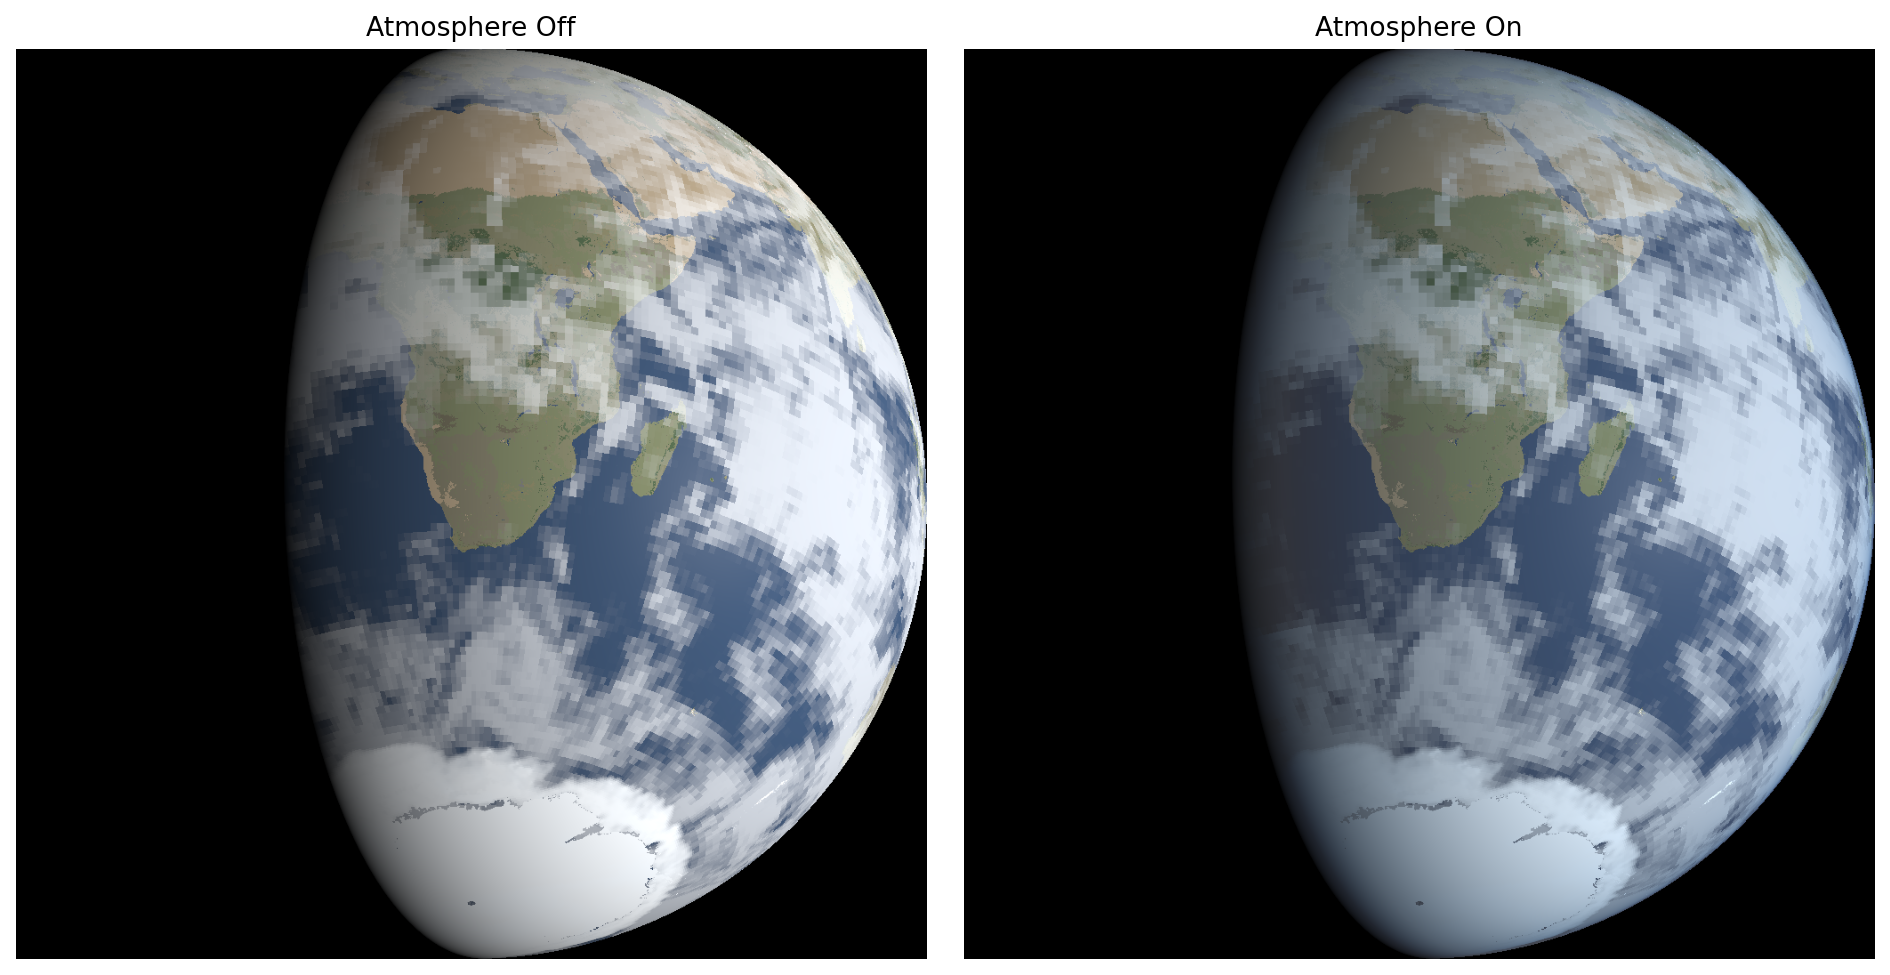
\includegraphics[width=0.98\textwidth]{fig/earth_atmosphere_compare.png}
  \caption{Comparison of atmosphere-off and atmosphere-on Earth renders from the current code. The atmosphere-on branch applies wavelength-dependent transmission and a single-scattered path-radiance term mixed between Rayleigh and aerosol phase functions.}
  \label{fig:atmcompare}
\end{figure}

\section{Colour Evolution Over Three Days}
To probe the time-dependent chromatic behaviour of the model, a three-day simulation was generated at a cadence of twenty minutes per frame, once with the atmosphere enabled and once with the atmosphere disabled. For each rendered Earth FITS cube, the summed radiances in the \texttt{RAD\_R}, \texttt{RAD\_G}, and \texttt{RAD\_B} layers were extracted from the FITS header. These time series were then reduced into broadband colour diagnostics in two equivalent forms: direct flux ratios such as \(R/G\), \(R/B\), and \(G/B\), and astronomical colour indices written as differences of magnitudes, such as \(m_R - m_G\), \(m_R - m_B\), and \(m_B - m_G\). The ratio form keeps the discussion in explicitly radiometric terms, while the colour-index form is often easier for astronomers to interpret because it compresses multiplicative changes into additive curves.

The scientific point of these plots is not merely that the model Earth brightens and fades. The more interesting quantity is the evolution of the colour-changing part of the system. As the Earth rotates, different combinations of land, ocean, cloud, sea ice, glint geometry, and atmospheric path radiance rotate into view. Those changes alter the relative channel balance, not just the total flux. In that sense the colour curves provide a compact diagnostic of the model physics: they reveal whether the renderer is producing time-variable chromatic structure that is plausibly tied to changing surface and atmospheric conditions rather than only a scalar modulation of brightness.

Figure~\ref{fig:ratio3d} shows the three-day sequence in terms of flux ratios. This presentation is natural for geophysical interpretation because it stays close to the underlying radiance sums. Figure~\ref{fig:colourindex3d} shows the same simulation expressed as colour indices in the astronomical sense. In both figures, the atmosphere-on and atmosphere-off branches are plotted on the same axes, and all panels within a figure share a common vertical scale. That makes it easier to judge not only whether the two branches differ, but also which colour combination is most sensitive to the atmospheric treatment.

\begin{figure}[p]
  \centering
  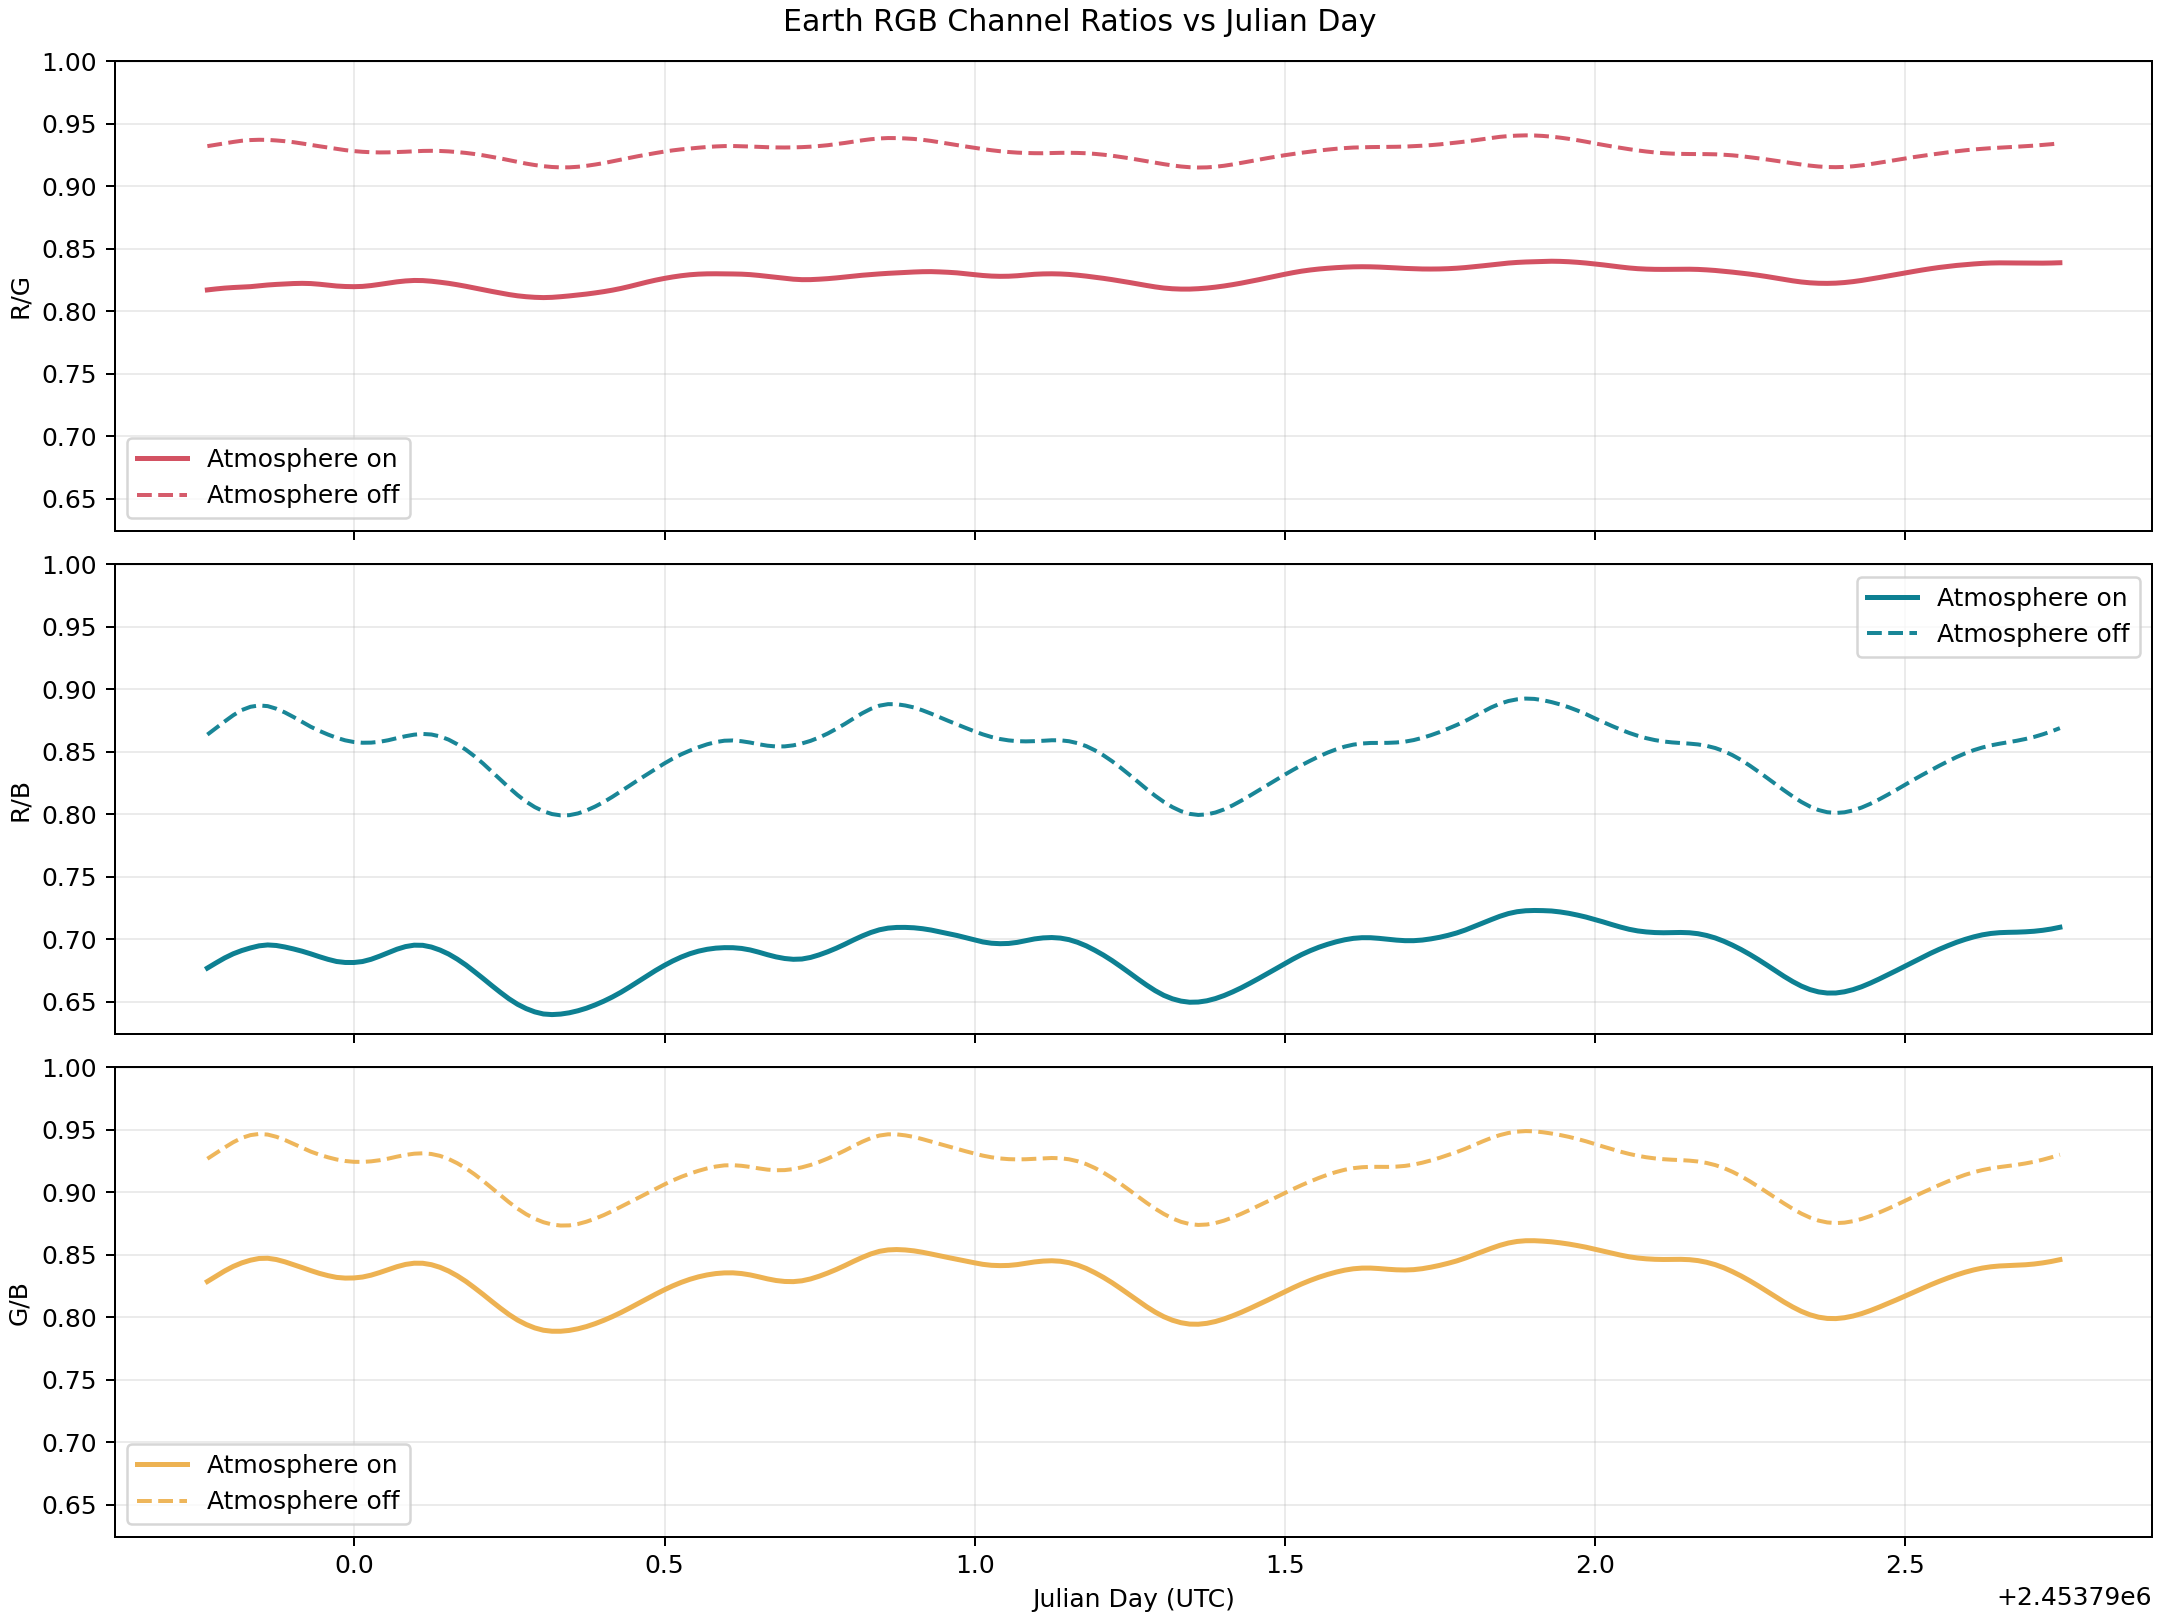
\includegraphics[width=0.98\textwidth]{fig/earth_rgb_ratios_3d_20min_ratio_combined.png}
  \caption{Three-day Earth simulation sampled every twenty minutes, plotted as broadband flux ratios derived from the summed \texttt{RAD\_R}, \texttt{RAD\_G}, and \texttt{RAD\_B} layers. The solid curves correspond to the atmosphere-on model and the dashed curves to the atmosphere-off model. Caption text to be refined after Overleaf upload.}
  \label{fig:ratio3d}
\end{figure}

\begin{figure}[p]
  \centering
  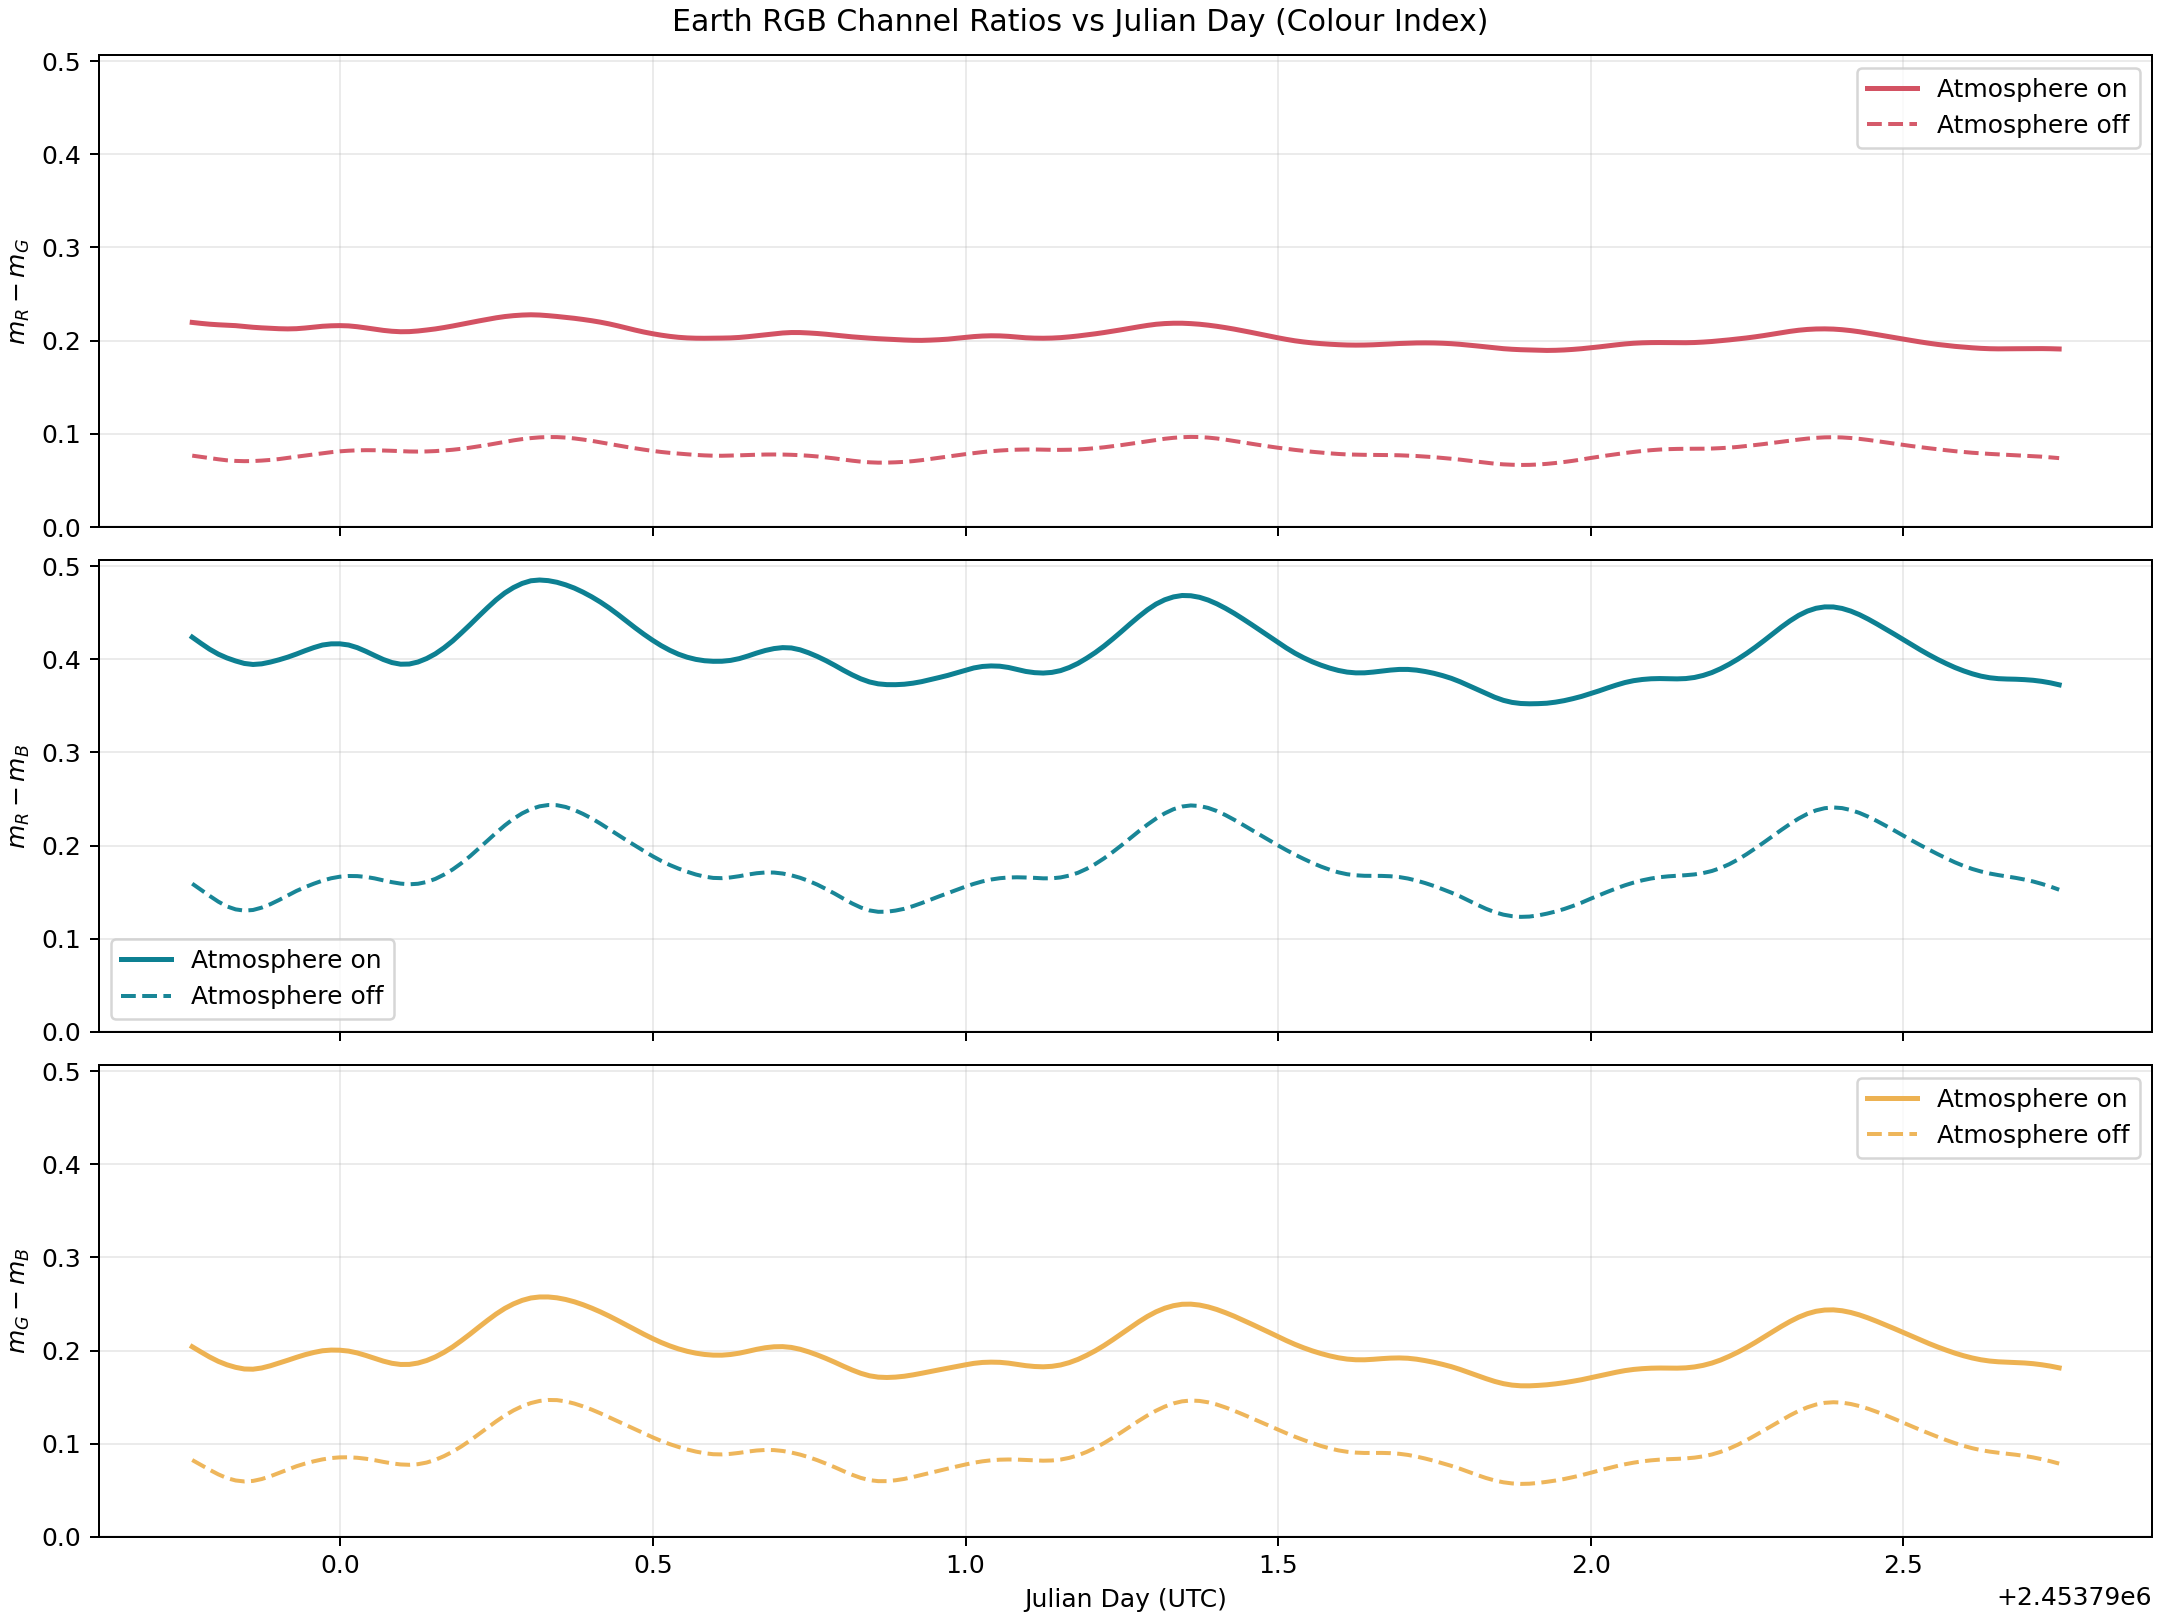
\includegraphics[width=0.98\textwidth]{fig/earth_rgb_ratios_3d_20min_mag_combined.png}
  \caption{The same three-day simulation expressed as colour indices, using astronomical notation \(m_R - m_G\), \(m_R - m_B\), and \(m_B - m_G\). This form emphasises chromatic evolution in a representation familiar to astronomers while remaining directly tied to the radiance ratios. Caption text to be refined after Overleaf upload.}
  \label{fig:colourindex3d}
\end{figure}

\section{Example Workflow}
It is useful to give one explicit example that corresponds directly to the comparison figure in this note. In the present workflow, the atmosphere is not toggled by a dedicated command-line flag. Instead, it is controlled from the configuration file through the \texttt{[earth]} block, in particular the keys \texttt{atmosphere\_enable}, \texttt{atmosphere\_strength}, \texttt{rayleigh\_tau\_rgb}, \texttt{aerosol\_tau\_rgb}, and \texttt{aerosol\_g}. A minimal example therefore starts by preparing one config file with \texttt{atmosphere\_enable = true} and another with \texttt{atmosphere\_enable = false}, then rendering the two Earth FITS products for the same Julian Day.

\begin{verbatim}
uv run python tools/render_earth_fits.py \
  --config /tmp/scene_atm_on.toml \
  --jd 2453789.7630208 \
  --out OUTPUT/earth_synth_jd2453789p7630208_atm_on.fits
\end{verbatim}

That command writes a FITS cube containing the monochrome radiance products, the RGB radiance layers, the atmospheric path-radiance layers, the transmission layers, the albedo layers, and the supporting diagnostics. In the current layer ordering, the RGB radiance planes are \texttt{RAD\_R}, \texttt{RAD\_G}, and \texttt{RAD\_B}. The comparison PNG was then made by extracting the RGB planes from the atmosphere-on and atmosphere-off outputs, converting them into display images, and combining them into one two-panel figure.

\begin{verbatim}
uv run python - <<'PY'
from astropy.io import fits
import matplotlib.pyplot as plt
import numpy as np

d = fits.getdata("OUTPUT/earth_synth_jd2453789p7630208_atm_on.fits")
r, g, b = d[5], d[6], d[7]
rgb = np.stack([r, g, b], axis=-1)
m = rgb.max()
if m > 0:
    rgb = rgb / m
plt.imsave("OUTPUT/earth_synth_jd2453789p7630208_atm_on.png", rgb.clip(0, 1))
PY
\end{verbatim}

This example is intentionally simple. It mirrors the exact development usage of the current code and makes clear that the displayed PNG is not a separate renderer output format. It is a visualisation product derived from the radiance layers in the FITS cube. The same pattern can be reused for atmosphere-off images, class-colour tests, or comparisons between alternative Earth configurations.

\section{Command-Line Interface}
The Earth renderer currently exposes the arguments below.

\begin{itemize}
  \item \texttt{--config PATH}. This selects the scene configuration file, defaulting to \texttt{scene.toml}. In practice this is the main control surface for the Earth model because almost all physically meaningful switches live in the \texttt{[earth]} block rather than on the command line. A different config can turn the atmosphere on or off, swap cloud maps, change the class map, change ice handling, alter glint parameters, or redirect the albedo map.
  \item \texttt{--utc ISO8601}. This overrides the timestamp from the config using an explicit UTC string such as \texttt{2006-02-17T06:18:45Z}. It is the clearest way to request a single render at a known instant. Because the Earth model uses SPICE geometry, changing this time changes both the illumination geometry and the observer-facing hemisphere.
  \item \texttt{--jd FLOAT}. This provides the time as a Julian Day on the UTC scale. It is an alternative to \texttt{--utc} and the two may not be used together. This argument is especially convenient when the Earth renderer is called from scripts that already work in JD space, for example when building evenly sampled sequences over long time ranges.
  \item \texttt{--out PATH}. This sets the output FITS filename explicitly. If omitted, the script constructs a timestamp-based name under \texttt{OUTPUT/}. In routine use this argument matters because the Earth renderer is often run repeatedly for atmosphere-on, atmosphere-off, colour, and diagnostic variants, and explicit filenames avoid accidental overwrites.
  \item \texttt{--nx INTEGER}. This sets the output image width in pixels. The default is 1024. Because the renderer works by sampling an orthographic disk on the image grid, increasing \texttt{--nx} directly increases the spatial resolution of the visible Earth disk and the cost of the render.
  \item \texttt{--ny INTEGER}. This sets the output image height in pixels. The default is 1024. In practice one normally keeps \texttt{--nx} and \texttt{--ny} equal so that the Earth disk remains circular and the pixel scale is isotropic, but the code does not require that symmetry.
  \item \texttt{--only-layer-index INTEGER}. This tells the renderer to write only a single layer from the internal layer list instead of the full 34-layer cube. The index is one-based. This is useful when a downstream tool wants only one radiance or I/F image and does not need the full diagnostic payload. When used on a physical layer, the output header also contains a \texttt{SUMPIX} keyword for the written plane.
  \item \texttt{--view \{moon\_center, earth\_site\}}. This chooses the viewpoint from which Earth is rendered. \texttt{moon\_center} renders Earth as seen from the Moon. \texttt{earth\_site} renders Earth as seen from a terrestrial observing site. The distinction is not cosmetic. It changes the observer position in inertial space and therefore changes the visible hemisphere and the Earth phase.
  \item \texttt{--lon FLOAT}. This gives observer longitude in degrees and is used only with \texttt{--view earth\_site}. It overrides the longitude in the config file. For Earth-site renders this parameter determines the local position whose topocentric viewpoint is used to look back at the Earth.
  \item \texttt{--lat FLOAT}. This gives observer latitude in degrees and is used only with \texttt{--view earth\_site}. Like longitude, it overrides the config file. Together with \texttt{--lon} and \texttt{--alt-m}, it defines the terrestrial site whose viewing geometry is transformed into J2000.
  \item \texttt{--alt-m FLOAT}. This gives observer altitude in metres and is used only with \texttt{--view earth\_site}. It completes the terrestrial site specification. While altitude is usually a small correction compared with the Earth radius, it is still part of the geometric definition and is therefore kept explicit in the interface.
\end{itemize}

\section{Current Limitations}
The present Earth model is already useful, but it is important to state what it is not. It is not a spectrally resolved model. It is not a multiple-scattering radiative transfer code. It does not carry a vertically resolved cloud model, and its atmosphere is intentionally first-order. The surface BRDF is Lambertian except for the glint increment applied over ocean. The class-based colour mapping is deterministic and practical, but not derived from a calibrated hyperspectral surface library. These are not hidden shortcomings. They are explicit design tradeoffs in service of a renderer that needs to run repeatedly inside a larger synthetic Moon and Earth workflow.

\section{Conclusion}
The current Earth renderer in \texttt{synthmoon} is best understood as a layered synthetic imaging model. SPICE provides geometry. Map products provide surface context. Class IDs provide robust land-cover colouring. Daily cloud and sea-ice products inject time dependence. Glint adds an important specular cue over oceans. A first-order atmosphere imposes wavelength-dependent attenuation and path radiance. The output cube then exposes both the finished image and the internal diagnostic components. That architecture is coherent, computationally manageable, and already rich enough to support both stand-alone Earth products and the Earth-facing parts of the broader Moon-rendering system.

\printbibliography

\end{document}
